
\chapter{2 Вводная электронная схема 15}

\section{2.1 Где купить комплектующие? 15}

В Новой Зеландии есть некоторое количество отличных поставщиков компонентов с
разумными ценами, включающих \url{www.surplustronics.co.nz}, и
\url{www.activecomponents.com}. Зарубежные поставщики, которых я использую,
включают \url{www.digikey.co.nz}, \url{www.sparkfun.com}, \url{ebay.com}
и \url{aliexpress.com}

\bigskip
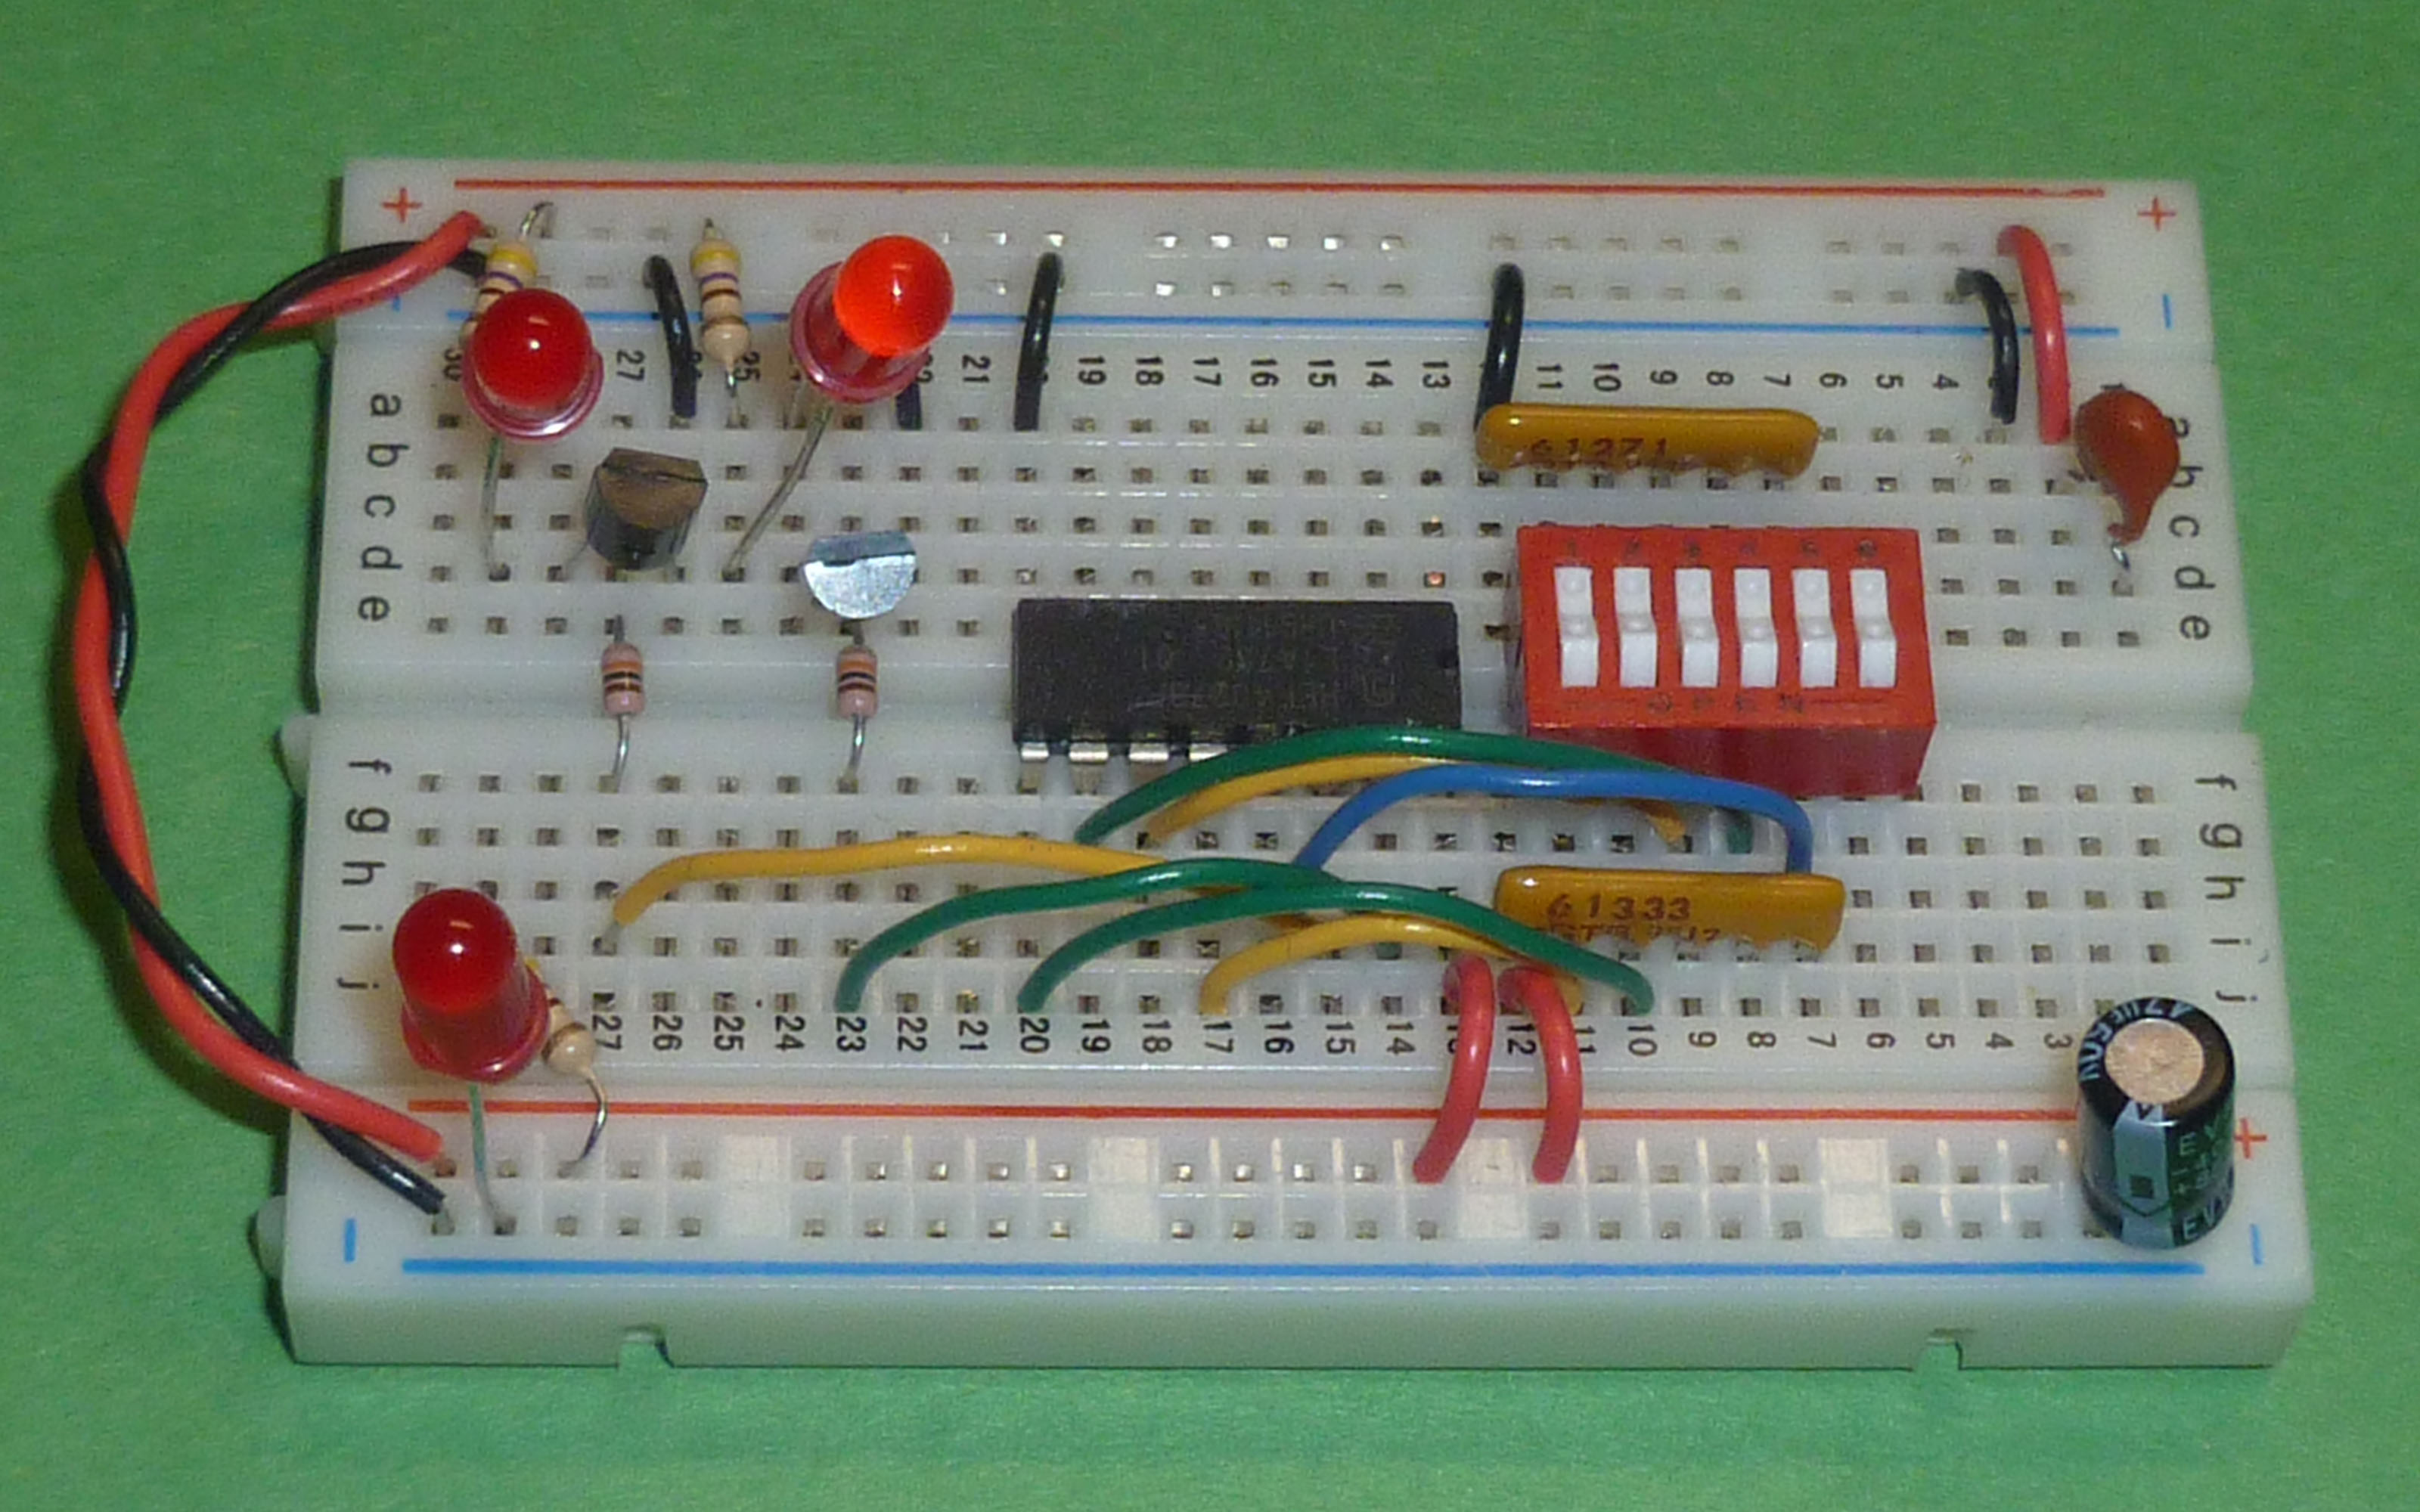
\includegraphics[width=0.8\textwidth]{bcollis/breadboard2.jpg}

Макетная плата (breadboard)\ --- пластмассовый блок с отверстиями и
металлическими полосковыми металлическими зажимами, создающими соединения между
элементами схемы. Отверстия расположены так, что компоненты могут быть соединены
вместе формируя схему. Верхние и нижние ряды, как правило, используется для шин
питания, красный сверху для плюса, и внизу черный/синий для для минуса (общий
провод).

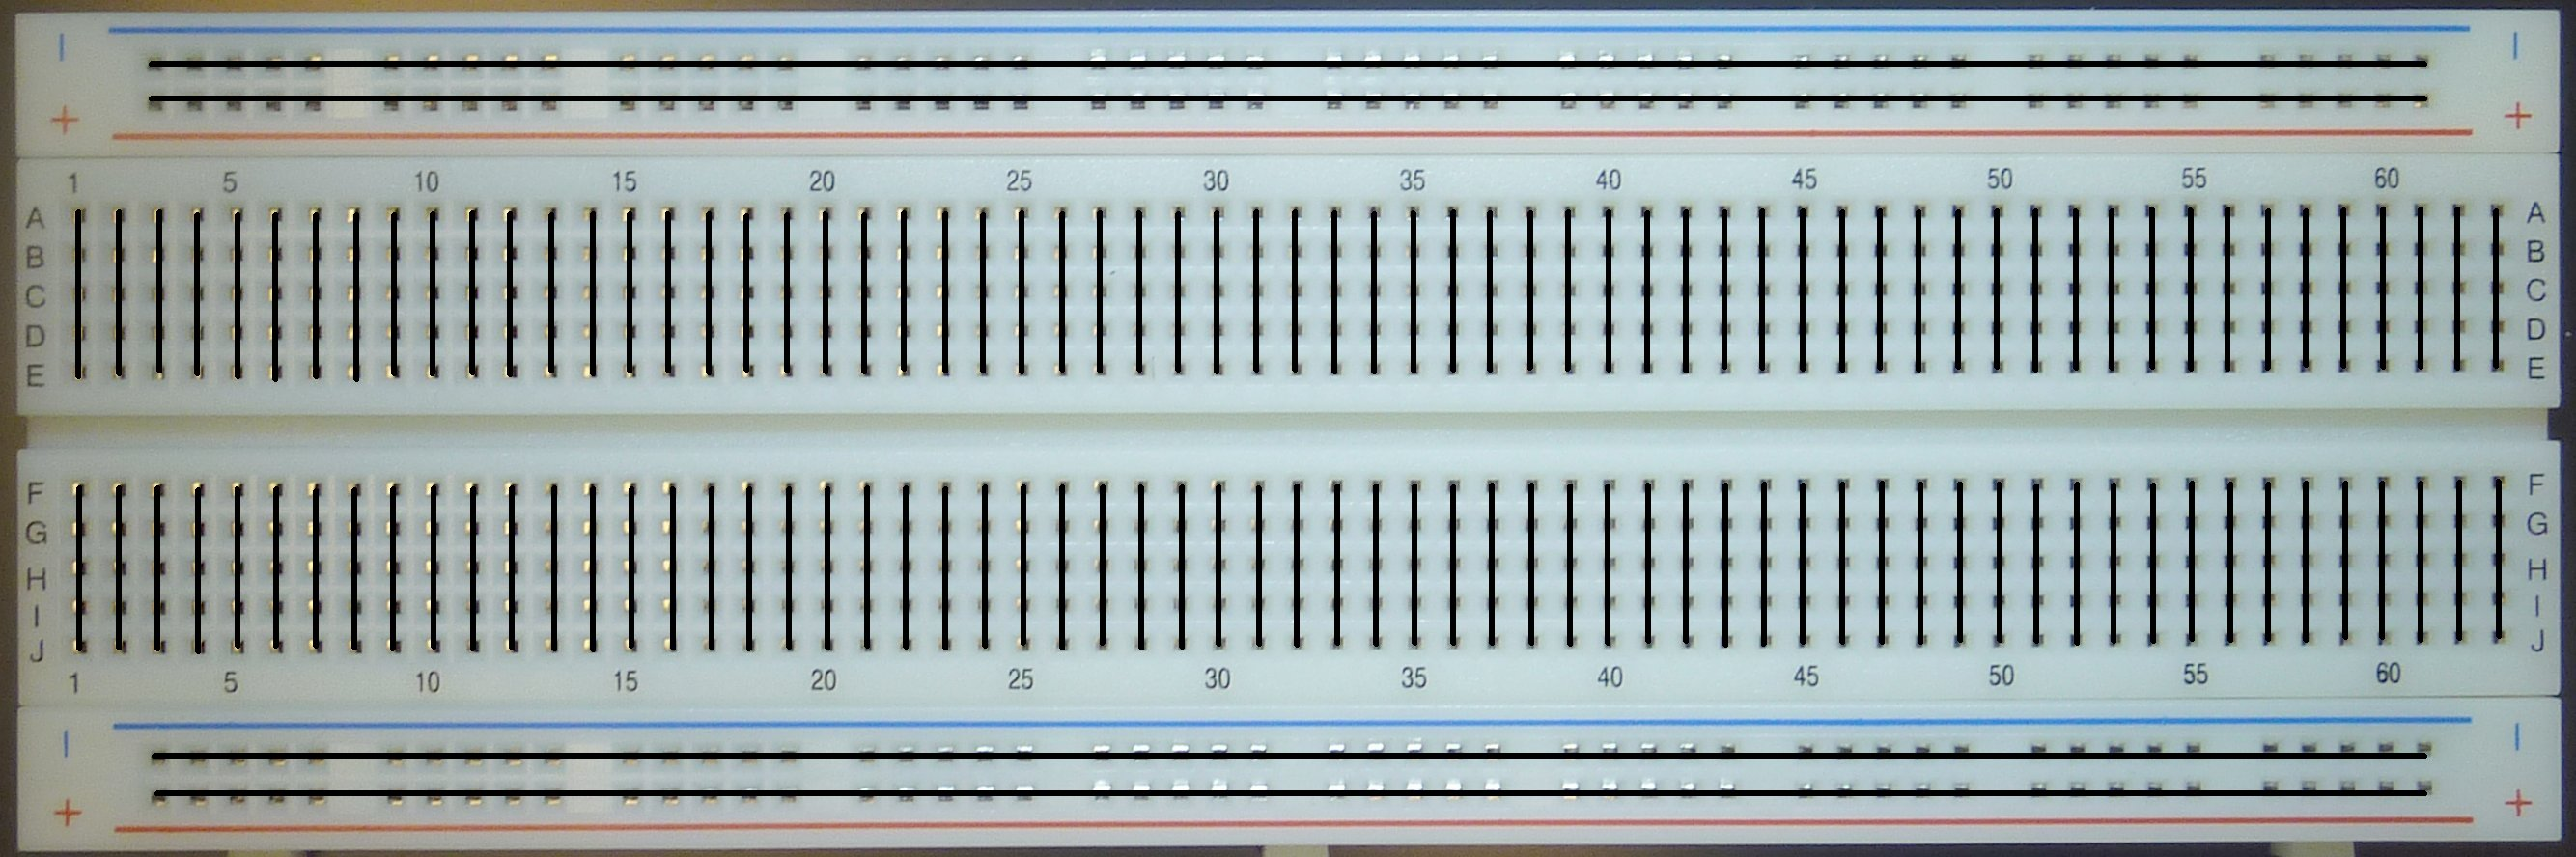
\includegraphics[width=0.8\textwidth]{bcollis/BreadboardConnections.jpg}

\bigskip

Эта схема \ref{ch21sch}\ может быть собрана вот так \ref{ch21lay}, обратите
внимание, что светодиод должен находиться в правильном положении. Если у вас
есть светодиод и резистор, соединенные в замкнутый контур, светодиод должен
загореться.

\bigskip
Принципиальная схема \label{ch21sch}

\bigskip
Компоновка \label{ch21lay}

\bigskip
The LED requires 2V the battery is 9V, if you put the LED across the battery it
would stop working! So a 1k (1000ohm) resistor is used to reduce the voltage to
the LED and the current through it, get a multimeter and measure the voltage
across the resistor, is it close to 7V? If you disconnect any wire within the
circuit it stops working, a circuit needs to be complete before electrons can
flow.

\section{2.2 Определение сопротивления резистора по цветовому коду 16}

.

\section{2.3 Светодиоды 17}

.

\section{2,4 Некоторые технические характеристики светодиода 17}

.

\section{2.5 Задание на исследование светодиода 17}

.

\section{2.6 Добавление выключателя  в схему 18}

.

\section{2.7 Задание на установку выключателя 18}

.

\section{2,8 Важные понятия схемы 19}

.

\section{2.9 Изменение величины сопротивления 19}

.

\section{2.10 Добавление транзистора в схему 20}

.

\section{2.11 Чтение схем 21}

.

\section{2.12 Входная цепь\ --- LDR 22}

.

\section{2.13 Рабочая схема датчика темноты 23}

.

\section{2,14 Защитные цепи - использование диода 24}

.

\section{2.15 Задача исследования диода 24}

.

\section{2.13 Финальная схема датчика темноты 23}

.

